% Options for packages loaded elsewhere
\PassOptionsToPackage{unicode}{hyperref}
\PassOptionsToPackage{hyphens}{url}
%
\documentclass[
]{article}
\usepackage{amsmath,amssymb}
\usepackage{lmodern}
\usepackage{iftex}
\ifPDFTeX
  \usepackage[T1]{fontenc}
  \usepackage[utf8]{inputenc}
  \usepackage{textcomp} % provide euro and other symbols
\else % if luatex or xetex
  \usepackage{unicode-math}
  \defaultfontfeatures{Scale=MatchLowercase}
  \defaultfontfeatures[\rmfamily]{Ligatures=TeX,Scale=1}
\fi
% Use upquote if available, for straight quotes in verbatim environments
\IfFileExists{upquote.sty}{\usepackage{upquote}}{}
\IfFileExists{microtype.sty}{% use microtype if available
  \usepackage[]{microtype}
  \UseMicrotypeSet[protrusion]{basicmath} % disable protrusion for tt fonts
}{}
\makeatletter
\@ifundefined{KOMAClassName}{% if non-KOMA class
  \IfFileExists{parskip.sty}{%
    \usepackage{parskip}
  }{% else
    \setlength{\parindent}{0pt}
    \setlength{\parskip}{6pt plus 2pt minus 1pt}}
}{% if KOMA class
  \KOMAoptions{parskip=half}}
\makeatother
\usepackage{xcolor}
\usepackage[margin=1in]{geometry}
\usepackage{color}
\usepackage{fancyvrb}
\newcommand{\VerbBar}{|}
\newcommand{\VERB}{\Verb[commandchars=\\\{\}]}
\DefineVerbatimEnvironment{Highlighting}{Verbatim}{commandchars=\\\{\}}
% Add ',fontsize=\small' for more characters per line
\usepackage{framed}
\definecolor{shadecolor}{RGB}{248,248,248}
\newenvironment{Shaded}{\begin{snugshade}}{\end{snugshade}}
\newcommand{\AlertTok}[1]{\textcolor[rgb]{0.94,0.16,0.16}{#1}}
\newcommand{\AnnotationTok}[1]{\textcolor[rgb]{0.56,0.35,0.01}{\textbf{\textit{#1}}}}
\newcommand{\AttributeTok}[1]{\textcolor[rgb]{0.77,0.63,0.00}{#1}}
\newcommand{\BaseNTok}[1]{\textcolor[rgb]{0.00,0.00,0.81}{#1}}
\newcommand{\BuiltInTok}[1]{#1}
\newcommand{\CharTok}[1]{\textcolor[rgb]{0.31,0.60,0.02}{#1}}
\newcommand{\CommentTok}[1]{\textcolor[rgb]{0.56,0.35,0.01}{\textit{#1}}}
\newcommand{\CommentVarTok}[1]{\textcolor[rgb]{0.56,0.35,0.01}{\textbf{\textit{#1}}}}
\newcommand{\ConstantTok}[1]{\textcolor[rgb]{0.00,0.00,0.00}{#1}}
\newcommand{\ControlFlowTok}[1]{\textcolor[rgb]{0.13,0.29,0.53}{\textbf{#1}}}
\newcommand{\DataTypeTok}[1]{\textcolor[rgb]{0.13,0.29,0.53}{#1}}
\newcommand{\DecValTok}[1]{\textcolor[rgb]{0.00,0.00,0.81}{#1}}
\newcommand{\DocumentationTok}[1]{\textcolor[rgb]{0.56,0.35,0.01}{\textbf{\textit{#1}}}}
\newcommand{\ErrorTok}[1]{\textcolor[rgb]{0.64,0.00,0.00}{\textbf{#1}}}
\newcommand{\ExtensionTok}[1]{#1}
\newcommand{\FloatTok}[1]{\textcolor[rgb]{0.00,0.00,0.81}{#1}}
\newcommand{\FunctionTok}[1]{\textcolor[rgb]{0.00,0.00,0.00}{#1}}
\newcommand{\ImportTok}[1]{#1}
\newcommand{\InformationTok}[1]{\textcolor[rgb]{0.56,0.35,0.01}{\textbf{\textit{#1}}}}
\newcommand{\KeywordTok}[1]{\textcolor[rgb]{0.13,0.29,0.53}{\textbf{#1}}}
\newcommand{\NormalTok}[1]{#1}
\newcommand{\OperatorTok}[1]{\textcolor[rgb]{0.81,0.36,0.00}{\textbf{#1}}}
\newcommand{\OtherTok}[1]{\textcolor[rgb]{0.56,0.35,0.01}{#1}}
\newcommand{\PreprocessorTok}[1]{\textcolor[rgb]{0.56,0.35,0.01}{\textit{#1}}}
\newcommand{\RegionMarkerTok}[1]{#1}
\newcommand{\SpecialCharTok}[1]{\textcolor[rgb]{0.00,0.00,0.00}{#1}}
\newcommand{\SpecialStringTok}[1]{\textcolor[rgb]{0.31,0.60,0.02}{#1}}
\newcommand{\StringTok}[1]{\textcolor[rgb]{0.31,0.60,0.02}{#1}}
\newcommand{\VariableTok}[1]{\textcolor[rgb]{0.00,0.00,0.00}{#1}}
\newcommand{\VerbatimStringTok}[1]{\textcolor[rgb]{0.31,0.60,0.02}{#1}}
\newcommand{\WarningTok}[1]{\textcolor[rgb]{0.56,0.35,0.01}{\textbf{\textit{#1}}}}
\usepackage{longtable,booktabs,array}
\usepackage{calc} % for calculating minipage widths
% Correct order of tables after \paragraph or \subparagraph
\usepackage{etoolbox}
\makeatletter
\patchcmd\longtable{\par}{\if@noskipsec\mbox{}\fi\par}{}{}
\makeatother
% Allow footnotes in longtable head/foot
\IfFileExists{footnotehyper.sty}{\usepackage{footnotehyper}}{\usepackage{footnote}}
\makesavenoteenv{longtable}
\usepackage{graphicx}
\makeatletter
\def\maxwidth{\ifdim\Gin@nat@width>\linewidth\linewidth\else\Gin@nat@width\fi}
\def\maxheight{\ifdim\Gin@nat@height>\textheight\textheight\else\Gin@nat@height\fi}
\makeatother
% Scale images if necessary, so that they will not overflow the page
% margins by default, and it is still possible to overwrite the defaults
% using explicit options in \includegraphics[width, height, ...]{}
\setkeys{Gin}{width=\maxwidth,height=\maxheight,keepaspectratio}
% Set default figure placement to htbp
\makeatletter
\def\fps@figure{htbp}
\makeatother
\setlength{\emergencystretch}{3em} % prevent overfull lines
\providecommand{\tightlist}{%
  \setlength{\itemsep}{0pt}\setlength{\parskip}{0pt}}
\setcounter{secnumdepth}{-\maxdimen} % remove section numbering
\ifLuaTeX
  \usepackage{selnolig}  % disable illegal ligatures
\fi
\IfFileExists{bookmark.sty}{\usepackage{bookmark}}{\usepackage{hyperref}}
\IfFileExists{xurl.sty}{\usepackage{xurl}}{} % add URL line breaks if available
\urlstyle{same} % disable monospaced font for URLs
\hypersetup{
  pdftitle={Logistic Regression Project},
  pdfauthor={Ian Mbaya},
  hidelinks,
  pdfcreator={LaTeX via pandoc}}

\title{Logistic Regression Project}
\author{Ian Mbaya}
\date{2024-04-25}

\begin{document}
\maketitle

\hypertarget{load-the-neccessary-libraries}{%
\subsection{Load the Neccessary
Libraries}\label{load-the-neccessary-libraries}}

\begin{Shaded}
\begin{Highlighting}[]
\FunctionTok{library}\NormalTok{(}\StringTok{\textquotesingle{}tidyverse\textquotesingle{}}\NormalTok{)}
\end{Highlighting}
\end{Shaded}

\begin{verbatim}
## -- Attaching core tidyverse packages ------------------------ tidyverse 2.0.0 --
## v dplyr     1.1.4     v readr     2.1.4
## v forcats   1.0.0     v stringr   1.5.0
## v ggplot2   3.4.2     v tibble    3.2.1
## v lubridate 1.9.2     v tidyr     1.3.0
## v purrr     1.0.1     
## -- Conflicts ------------------------------------------ tidyverse_conflicts() --
## x dplyr::filter() masks stats::filter()
## x dplyr::lag()    masks stats::lag()
## i Use the conflicted package (<http://conflicted.r-lib.org/>) to force all conflicts to become errors
\end{verbatim}

\begin{Shaded}
\begin{Highlighting}[]
\FunctionTok{library}\NormalTok{(}\StringTok{\textquotesingle{}tidymodels\textquotesingle{}}\NormalTok{)}
\end{Highlighting}
\end{Shaded}

\begin{verbatim}
## -- Attaching packages -------------------------------------- tidymodels 1.1.0 --
## v broom        1.0.5     v rsample      1.1.1
## v dials        1.2.0     v tune         1.1.1
## v infer        1.0.4     v workflows    1.1.3
## v modeldata    1.1.0     v workflowsets 1.0.1
## v parsnip      1.1.1     v yardstick    1.2.0
## v recipes      1.0.6     
## -- Conflicts ----------------------------------------- tidymodels_conflicts() --
## x scales::discard() masks purrr::discard()
## x dplyr::filter()   masks stats::filter()
## x recipes::fixed()  masks stringr::fixed()
## x dplyr::lag()      masks stats::lag()
## x yardstick::spec() masks readr::spec()
## x recipes::step()   masks stats::step()
## * Use tidymodels_prefer() to resolve common conflicts.
\end{verbatim}

\begin{Shaded}
\begin{Highlighting}[]
\FunctionTok{library}\NormalTok{(}\StringTok{\textquotesingle{}caret\textquotesingle{}}\NormalTok{)}
\end{Highlighting}
\end{Shaded}

\begin{verbatim}
## Loading required package: lattice
## 
## Attaching package: 'caret'
## 
## The following objects are masked from 'package:yardstick':
## 
##     precision, recall, sensitivity, specificity
## 
## The following object is masked from 'package:purrr':
## 
##     lift
\end{verbatim}

\begin{Shaded}
\begin{Highlighting}[]
\FunctionTok{library}\NormalTok{(}\StringTok{\textquotesingle{}pROC\textquotesingle{}}\NormalTok{)}
\end{Highlighting}
\end{Shaded}

\begin{verbatim}
## Type 'citation("pROC")' for a citation.
## 
## Attaching package: 'pROC'
## 
## The following objects are masked from 'package:stats':
## 
##     cov, smooth, var
\end{verbatim}

\begin{Shaded}
\begin{Highlighting}[]
\FunctionTok{library}\NormalTok{(}\StringTok{\textquotesingle{}lubridate\textquotesingle{}}\NormalTok{)}
\FunctionTok{library}\NormalTok{(}\StringTok{\textquotesingle{}writexl\textquotesingle{}}\NormalTok{)}
\FunctionTok{library}\NormalTok{(}\StringTok{\textquotesingle{}knitr\textquotesingle{}}\NormalTok{)}
\end{Highlighting}
\end{Shaded}

\hypertarget{loading-the-data}{%
\section{Loading the Data}\label{loading-the-data}}

\hypertarget{i-am-using-data1-because-of-size-constraints.-the-original-file-was-too-big-for-github}{%
\subsection{I am using data1 because of size constraints. The original
file was too big for
github}\label{i-am-using-data1-because-of-size-constraints.-the-original-file-was-too-big-for-github}}

\begin{Shaded}
\begin{Highlighting}[]
\CommentTok{\#attacks \textless{}{-} read.csv("data/CTU1.csv", sep = "|") Deleted File}
\NormalTok{attacks }\OtherTok{\textless{}{-}}\NormalTok{ readxl}\SpecialCharTok{::}\FunctionTok{read\_xlsx}\NormalTok{(}\StringTok{"data/data1.xlsx"}\NormalTok{)}
\end{Highlighting}
\end{Shaded}

\hypertarget{preliminary-data-analysis}{%
\section{Preliminary Data Analysis}\label{preliminary-data-analysis}}

\hypertarget{take-a-glimpse-of-the-data}{%
\subsection{Take a Glimpse of the
Data}\label{take-a-glimpse-of-the-data}}

\begin{Shaded}
\begin{Highlighting}[]
\NormalTok{dplyr}\SpecialCharTok{::}\FunctionTok{glimpse}\NormalTok{(attacks)}
\end{Highlighting}
\end{Shaded}

\begin{verbatim}
## Rows: 1,008,748
## Columns: 8
## $ label         <chr> "Malicious", "Malicious", "Malicious", "Malicious", "Mal~
## $ ts            <dttm> 2018-05-09 15:30:31, 2018-05-09 15:30:31, 2018-05-09 15~
## $ id.resp_h     <chr> "65.127.233.163", "63.150.16.171", "111.40.23.49", "131.~
## $ id.resp_p     <dbl> 23, 23, 23, 23, 23, 23, 49560, 21288, 23, 8080, 8080, 23~
## $ id.orig_p     <dbl> 51524, 56305, 41101, 60905, 44301, 50244, 34243, 34840, ~
## $ proto         <chr> "tcp", "tcp", "tcp", "tcp", "tcp", "tcp", "tcp", "tcp", ~
## $ history       <chr> "S", "S", "S", "S", "S", "S", "S", "S", "S", "S", "S", "~
## $ orig_ip_bytes <dbl> 180, 60, 60, 180, 60, 60, 180, 60, 60, 60, 60, 180, 180,~
\end{verbatim}

\hypertarget{data-summary}{%
\subsection{Data Summary}\label{data-summary}}

\begin{Shaded}
\begin{Highlighting}[]
\FunctionTok{summary}\NormalTok{(attacks)}
\end{Highlighting}
\end{Shaded}

\begin{verbatim}
##     label                 ts                          id.resp_h        
##  Length:1008748     Min.   :2018-05-09 15:30:31.01   Length:1008748    
##  Class :character   1st Qu.:2018-05-10 17:57:40.75   Class :character  
##  Mode  :character   Median :2018-05-11 20:40:00.00   Mode  :character  
##                     Mean   :2018-05-11 21:43:27.22                     
##                     3rd Qu.:2018-05-13 01:13:40.00                     
##                     Max.   :2018-05-14 07:24:43.02                     
##    id.resp_p       id.orig_p        proto             history         
##  Min.   :    0   Min.   :    3   Length:1008748     Length:1008748    
##  1st Qu.:   23   1st Qu.:43730   Class :character   Class :character  
##  Median : 8080   Median :43763   Mode  :character   Mode  :character  
##  Mean   :16098   Mean   :44437                                        
##  3rd Qu.:28180   3rd Qu.:48814                                        
##  Max.   :65535   Max.   :65394                                        
##  orig_ip_bytes    
##  Min.   :   0.00  
##  1st Qu.:  40.00  
##  Median :  60.00  
##  Mean   :  81.15  
##  3rd Qu.:  60.00  
##  Max.   :2990.00
\end{verbatim}

\hypertarget{checking-for-missing-values}{%
\subsection{Checking for Missing
Values}\label{checking-for-missing-values}}

\begin{Shaded}
\begin{Highlighting}[]
\NormalTok{skimr}\SpecialCharTok{::}\FunctionTok{skim}\NormalTok{(attacks)}
\end{Highlighting}
\end{Shaded}

\begin{longtable}[]{@{}ll@{}}
\caption{Data summary}\tabularnewline
\toprule()
\endhead
Name & attacks \\
Number of rows & 1008748 \\
Number of columns & 8 \\
\_\_\_\_\_\_\_\_\_\_\_\_\_\_\_\_\_\_\_\_\_\_\_ & \\
Column type frequency: & \\
character & 4 \\
numeric & 3 \\
POSIXct & 1 \\
\_\_\_\_\_\_\_\_\_\_\_\_\_\_\_\_\_\_\_\_\_\_\_\_ & \\
Group variables & None \\
\bottomrule()
\end{longtable}

\textbf{Variable type: character}

\begin{longtable}[]{@{}
  >{\raggedright\arraybackslash}p{(\columnwidth - 14\tabcolsep) * \real{0.1944}}
  >{\raggedleft\arraybackslash}p{(\columnwidth - 14\tabcolsep) * \real{0.1389}}
  >{\raggedleft\arraybackslash}p{(\columnwidth - 14\tabcolsep) * \real{0.1944}}
  >{\raggedleft\arraybackslash}p{(\columnwidth - 14\tabcolsep) * \real{0.0556}}
  >{\raggedleft\arraybackslash}p{(\columnwidth - 14\tabcolsep) * \real{0.0556}}
  >{\raggedleft\arraybackslash}p{(\columnwidth - 14\tabcolsep) * \real{0.0833}}
  >{\raggedleft\arraybackslash}p{(\columnwidth - 14\tabcolsep) * \real{0.1250}}
  >{\raggedleft\arraybackslash}p{(\columnwidth - 14\tabcolsep) * \real{0.1528}}@{}}
\toprule()
\begin{minipage}[b]{\linewidth}\raggedright
skim\_variable
\end{minipage} & \begin{minipage}[b]{\linewidth}\raggedleft
n\_missing
\end{minipage} & \begin{minipage}[b]{\linewidth}\raggedleft
complete\_rate
\end{minipage} & \begin{minipage}[b]{\linewidth}\raggedleft
min
\end{minipage} & \begin{minipage}[b]{\linewidth}\raggedleft
max
\end{minipage} & \begin{minipage}[b]{\linewidth}\raggedleft
empty
\end{minipage} & \begin{minipage}[b]{\linewidth}\raggedleft
n\_unique
\end{minipage} & \begin{minipage}[b]{\linewidth}\raggedleft
whitespace
\end{minipage} \\
\midrule()
\endhead
label & 0 & 1 & 6 & 9 & 0 & 2 & 0 \\
id.resp\_h & 0 & 1 & 7 & 15 & 0 & 597107 & 0 \\
proto & 0 & 1 & 3 & 4 & 0 & 3 & 0 \\
history & 0 & 1 & 1 & 10 & 0 & 126 & 0 \\
\bottomrule()
\end{longtable}

\textbf{Variable type: numeric}

\begin{longtable}[]{@{}
  >{\raggedright\arraybackslash}p{(\columnwidth - 20\tabcolsep) * \real{0.1522}}
  >{\raggedleft\arraybackslash}p{(\columnwidth - 20\tabcolsep) * \real{0.1087}}
  >{\raggedleft\arraybackslash}p{(\columnwidth - 20\tabcolsep) * \real{0.1522}}
  >{\raggedleft\arraybackslash}p{(\columnwidth - 20\tabcolsep) * \real{0.0978}}
  >{\raggedleft\arraybackslash}p{(\columnwidth - 20\tabcolsep) * \real{0.0978}}
  >{\raggedleft\arraybackslash}p{(\columnwidth - 20\tabcolsep) * \real{0.0326}}
  >{\raggedleft\arraybackslash}p{(\columnwidth - 20\tabcolsep) * \real{0.0652}}
  >{\raggedleft\arraybackslash}p{(\columnwidth - 20\tabcolsep) * \real{0.0652}}
  >{\raggedleft\arraybackslash}p{(\columnwidth - 20\tabcolsep) * \real{0.0978}}
  >{\raggedleft\arraybackslash}p{(\columnwidth - 20\tabcolsep) * \real{0.0652}}
  >{\raggedright\arraybackslash}p{(\columnwidth - 20\tabcolsep) * \real{0.0652}}@{}}
\toprule()
\begin{minipage}[b]{\linewidth}\raggedright
skim\_variable
\end{minipage} & \begin{minipage}[b]{\linewidth}\raggedleft
n\_missing
\end{minipage} & \begin{minipage}[b]{\linewidth}\raggedleft
complete\_rate
\end{minipage} & \begin{minipage}[b]{\linewidth}\raggedleft
mean
\end{minipage} & \begin{minipage}[b]{\linewidth}\raggedleft
sd
\end{minipage} & \begin{minipage}[b]{\linewidth}\raggedleft
p0
\end{minipage} & \begin{minipage}[b]{\linewidth}\raggedleft
p25
\end{minipage} & \begin{minipage}[b]{\linewidth}\raggedleft
p50
\end{minipage} & \begin{minipage}[b]{\linewidth}\raggedleft
p75
\end{minipage} & \begin{minipage}[b]{\linewidth}\raggedleft
p100
\end{minipage} & \begin{minipage}[b]{\linewidth}\raggedright
hist
\end{minipage} \\
\midrule()
\endhead
id.resp\_p & 0 & 1 & 16097.71 & 19562.80 & 0 & 23 & 8080 & 28180.25 &
65535 & ▇▁▁▁▁ \\
id.orig\_p & 0 & 1 & 44436.84 & 9660.59 & 3 & 43730 & 43763 & 48814.00 &
65394 & ▁▁▂▇▂ \\
orig\_ip\_bytes & 0 & 1 & 81.15 & 94.73 & 0 & 40 & 60 & 60.00 & 2990 &
▇▁▁▁▁ \\
\bottomrule()
\end{longtable}

\textbf{Variable type: POSIXct}

\begin{longtable}[]{@{}
  >{\raggedright\arraybackslash}p{(\columnwidth - 12\tabcolsep) * \real{0.1308}}
  >{\raggedleft\arraybackslash}p{(\columnwidth - 12\tabcolsep) * \real{0.0935}}
  >{\raggedleft\arraybackslash}p{(\columnwidth - 12\tabcolsep) * \real{0.1308}}
  >{\raggedright\arraybackslash}p{(\columnwidth - 12\tabcolsep) * \real{0.1869}}
  >{\raggedright\arraybackslash}p{(\columnwidth - 12\tabcolsep) * \real{0.1869}}
  >{\raggedright\arraybackslash}p{(\columnwidth - 12\tabcolsep) * \real{0.1869}}
  >{\raggedleft\arraybackslash}p{(\columnwidth - 12\tabcolsep) * \real{0.0841}}@{}}
\toprule()
\begin{minipage}[b]{\linewidth}\raggedright
skim\_variable
\end{minipage} & \begin{minipage}[b]{\linewidth}\raggedleft
n\_missing
\end{minipage} & \begin{minipage}[b]{\linewidth}\raggedleft
complete\_rate
\end{minipage} & \begin{minipage}[b]{\linewidth}\raggedright
min
\end{minipage} & \begin{minipage}[b]{\linewidth}\raggedright
max
\end{minipage} & \begin{minipage}[b]{\linewidth}\raggedright
median
\end{minipage} & \begin{minipage}[b]{\linewidth}\raggedleft
n\_unique
\end{minipage} \\
\midrule()
\endhead
ts & 0 & 1 & 2018-05-09 15:30:31 & 2018-05-14 07:24:43 & 2018-05-11
20:40:00 & 946455 \\
\bottomrule()
\end{longtable}

\hypertarget{create-a-data-dictionary}{%
\subsection{Create a Data Dictionary}\label{create-a-data-dictionary}}

\begin{Shaded}
\begin{Highlighting}[]
\CommentTok{\# Data Dictionary for Network Connection Data}
\NormalTok{data\_dictionary }\OtherTok{\textless{}{-}}\NormalTok{ tibble}\SpecialCharTok{::}\FunctionTok{tribble}\NormalTok{(}
  \SpecialCharTok{\textasciitilde{}}\NormalTok{Field\_Name,     }\SpecialCharTok{\textasciitilde{}}\NormalTok{Description,                                   }\SpecialCharTok{\textasciitilde{}}\NormalTok{Type,}
  \StringTok{"ts"}\NormalTok{,            }\StringTok{"The timestamp of the connection event."}\NormalTok{,      }\StringTok{"time"}\NormalTok{,}
  \StringTok{"uid"}\NormalTok{,           }\StringTok{"A unique identifier for the connection."}\NormalTok{,     }\StringTok{"string"}\NormalTok{,}
  \StringTok{"id.orig\_h"}\NormalTok{,     }\StringTok{"The source IP address."}\NormalTok{,                      }\StringTok{"addr"}\NormalTok{,}
  \StringTok{"id.orig\_p"}\NormalTok{,     }\StringTok{"The source port."}\NormalTok{,                            }\StringTok{"port"}\NormalTok{,}
  \StringTok{"id.resp\_h"}\NormalTok{,     }\StringTok{"The destination IP address."}\NormalTok{,                 }\StringTok{"addr"}\NormalTok{,}
  \StringTok{"id.resp\_p"}\NormalTok{,     }\StringTok{"The destination port."}\NormalTok{,                       }\StringTok{"port"}\NormalTok{,}
  \StringTok{"proto"}\NormalTok{,         }\StringTok{"The network protocol used (e.g., \textquotesingle{}tcp\textquotesingle{})."}\NormalTok{,    }\StringTok{"enum"}\NormalTok{,}
  \StringTok{"service"}\NormalTok{,       }\StringTok{"The service associated with the connection."}\NormalTok{, }\StringTok{"string"}\NormalTok{,}
  \StringTok{"duration"}\NormalTok{,      }\StringTok{"The duration of the connection."}\NormalTok{,             }\StringTok{"interval"}\NormalTok{,}
  \StringTok{"orig\_bytes"}\NormalTok{,    }\StringTok{"The number of bytes sent from the source to the destination."}\NormalTok{, }\StringTok{"count"}\NormalTok{,}
  \StringTok{"resp\_bytes"}\NormalTok{,    }\StringTok{"The number of bytes sent from the destination to the source."}\NormalTok{, }\StringTok{"count"}\NormalTok{,}
  \StringTok{"conn\_state"}\NormalTok{,    }\StringTok{"The state of the connection."}\NormalTok{,                }\StringTok{"string"}\NormalTok{,}
  \StringTok{"local\_orig"}\NormalTok{,    }\StringTok{"Indicates whether the connection is considered local or not."}\NormalTok{, }\StringTok{"bool"}\NormalTok{,}
  \StringTok{"local\_resp"}\NormalTok{,    }\StringTok{"Indicates whether the connection is considered local or not."}\NormalTok{, }\StringTok{"bool"}\NormalTok{,}
  \StringTok{"missed\_bytes"}\NormalTok{,  }\StringTok{"The number of missed bytes in the connection."}\NormalTok{, }\StringTok{"count"}\NormalTok{,}
  \StringTok{"history"}\NormalTok{,       }\StringTok{"A history of connection states."}\NormalTok{,             }\StringTok{"string"}\NormalTok{,}
  \StringTok{"orig\_pkts"}\NormalTok{,     }\StringTok{"The number of packets sent from the source to the destination."}\NormalTok{, }\StringTok{"count"}\NormalTok{,}
  \StringTok{"orig\_ip\_bytes"}\NormalTok{, }\StringTok{"The number of IP bytes sent from the source to the destination."}\NormalTok{, }\StringTok{"count"}\NormalTok{,}
  \StringTok{"resp\_pkts"}\NormalTok{,     }\StringTok{"The number of packets sent from the destination to the source."}\NormalTok{, }\StringTok{"count"}\NormalTok{,}
  \StringTok{"resp\_ip\_bytes"}\NormalTok{, }\StringTok{"The number of IP bytes sent from the destination to the source."}\NormalTok{, }\StringTok{"count"}\NormalTok{,}
  \StringTok{"tunnel\_parents"}\NormalTok{,}\StringTok{"Indicates if this connection is part of a tunnel."}\NormalTok{, }\StringTok{"set[string]"}\NormalTok{,}
  \StringTok{"label"}\NormalTok{,         }\StringTok{"A label associated with the connection (e.g., \textquotesingle{}Malicious\textquotesingle{} or \textquotesingle{}Benign\textquotesingle{})."}\NormalTok{, }\StringTok{"string"}\NormalTok{,}
  \StringTok{"detailed\_label"}\NormalTok{,}\StringTok{"A more detailed description or label for the connection."}\NormalTok{, }\StringTok{"string"}
\NormalTok{)}
\end{Highlighting}
\end{Shaded}

From the summary and glimpse functions above it seems like we might have
too many variables that may not be contributing to the model. While the
skim functions shows that there are no missing values some of the
variables have a dash has placeholder ``-''. In the following steps we
will be further exploring and visualizing the data to identify trends
and patterns in the data that will determine the most important
variables for prediction.

\hypertarget{data-processing-exploration-feature-engineering.}{%
\section{Data Processing, Exploration Feature
Engineering.}\label{data-processing-exploration-feature-engineering.}}

\hypertarget{correlation-analysis}{%
\subsection{Correlation Analysis}\label{correlation-analysis}}

Running A Correlation Analysis to Identify the variables that have the
highest corellation with network traffic label.

\begin{Shaded}
\begin{Highlighting}[]
\CommentTok{\# Check the levels of the label variable}
\FunctionTok{levels}\NormalTok{(attacks}\SpecialCharTok{$}\NormalTok{label)}
\end{Highlighting}
\end{Shaded}

\begin{verbatim}
## NULL
\end{verbatim}

\begin{Shaded}
\begin{Highlighting}[]
\CommentTok{\# Convert label to a factor if it\textquotesingle{}s not already}
\NormalTok{attacks}\SpecialCharTok{$}\NormalTok{label }\OtherTok{\textless{}{-}} \FunctionTok{as.factor}\NormalTok{(attacks}\SpecialCharTok{$}\NormalTok{label)}

\CommentTok{\# Calculate correlation using Cramér\textquotesingle{}s V for categorical variables}
\NormalTok{cramer\_v }\OtherTok{\textless{}{-}} \ControlFlowTok{function}\NormalTok{(x, y) \{}
\NormalTok{  confusion\_matrix }\OtherTok{\textless{}{-}} \FunctionTok{table}\NormalTok{(x, y)}
\NormalTok{  n }\OtherTok{\textless{}{-}} \FunctionTok{sum}\NormalTok{(confusion\_matrix)}
\NormalTok{  chi\_sq }\OtherTok{\textless{}{-}} \FunctionTok{chisq.test}\NormalTok{(confusion\_matrix)}\SpecialCharTok{$}\NormalTok{statistic}
  \FunctionTok{return}\NormalTok{(}\FunctionTok{sqrt}\NormalTok{(chi\_sq }\SpecialCharTok{/}\NormalTok{ (n }\SpecialCharTok{*}\NormalTok{ (}\FunctionTok{min}\NormalTok{(}\FunctionTok{nrow}\NormalTok{(confusion\_matrix), }\FunctionTok{ncol}\NormalTok{(confusion\_matrix)) }\SpecialCharTok{{-}} \DecValTok{1}\NormalTok{))))}
\NormalTok{\}}

\CommentTok{\# Calculate correlation between label and each categorical variable}
\NormalTok{correlation\_results }\OtherTok{\textless{}{-}} \FunctionTok{lapply}\NormalTok{(attacks[, }\SpecialCharTok{{-}}\FunctionTok{which}\NormalTok{(}\FunctionTok{names}\NormalTok{(attacks) }\SpecialCharTok{==} \StringTok{"label"}\NormalTok{)], cramer\_v, }\AttributeTok{y =}\NormalTok{ attacks}\SpecialCharTok{$}\NormalTok{label)}
\end{Highlighting}
\end{Shaded}

\begin{verbatim}
## Warning in chisq.test(confusion_matrix): Chi-squared approximation may be
## incorrect

## Warning in chisq.test(confusion_matrix): Chi-squared approximation may be
## incorrect

## Warning in chisq.test(confusion_matrix): Chi-squared approximation may be
## incorrect

## Warning in chisq.test(confusion_matrix): Chi-squared approximation may be
## incorrect

## Warning in chisq.test(confusion_matrix): Chi-squared approximation may be
## incorrect

## Warning in chisq.test(confusion_matrix): Chi-squared approximation may be
## incorrect
\end{verbatim}

\begin{Shaded}
\begin{Highlighting}[]
\CommentTok{\# Convert the results to a data frame}
\NormalTok{correlation\_df }\OtherTok{\textless{}{-}} \FunctionTok{data.frame}\NormalTok{(}
  \AttributeTok{variable =} \FunctionTok{names}\NormalTok{(correlation\_results),}
  \AttributeTok{correlation =} \FunctionTok{unlist}\NormalTok{(correlation\_results)}
\NormalTok{)}

\CommentTok{\# Visualize correlation}
\FunctionTok{ggplot}\NormalTok{(correlation\_df, }\FunctionTok{aes}\NormalTok{(}\AttributeTok{x =} \FunctionTok{reorder}\NormalTok{(variable, correlation), }\AttributeTok{y =}\NormalTok{ correlation)) }\SpecialCharTok{+}
  \FunctionTok{geom\_bar}\NormalTok{(}\AttributeTok{stat =} \StringTok{"identity"}\NormalTok{, }\AttributeTok{fill =} \StringTok{"skyblue"}\NormalTok{, }\AttributeTok{color =} \StringTok{"black"}\NormalTok{) }\SpecialCharTok{+}
  \FunctionTok{coord\_flip}\NormalTok{() }\SpecialCharTok{+}
  \FunctionTok{labs}\NormalTok{(}\AttributeTok{x =} \StringTok{"Variable"}\NormalTok{, }\AttributeTok{y =} \StringTok{"Correlation (Cramér\textquotesingle{}s V)"}\NormalTok{,}
       \AttributeTok{title =} \StringTok{"Correlation between Variables and Label"}\NormalTok{) }\SpecialCharTok{+}
  \FunctionTok{theme\_minimal}\NormalTok{()}
\end{Highlighting}
\end{Shaded}

\includegraphics{Notebook_files/figure-latex/unnamed-chunk-4-1.pdf}

\hypertarget{visualizing-pattern-in-network-traffic-based-on-timestamps}{%
\subsection{Visualizing Pattern in Network Traffic based on
Timestamps}\label{visualizing-pattern-in-network-traffic-based-on-timestamps}}

\begin{Shaded}
\begin{Highlighting}[]
\CommentTok{\# Convert \textquotesingle{}ts\textquotesingle{} to a DateTime object }
\NormalTok{attacks}\SpecialCharTok{$}\NormalTok{ts }\OtherTok{\textless{}{-}} \FunctionTok{as.POSIXct}\NormalTok{(attacks}\SpecialCharTok{$}\NormalTok{ts, }\AttributeTok{format =} \StringTok{"\%Y{-}\%m{-}\%d \%H:\%M:\%S"}\NormalTok{)  }

\CommentTok{\# Create a new dataframe with counts of attacks per time period (e.g., per day)}
\NormalTok{attacks\_per\_period }\OtherTok{\textless{}{-}}\NormalTok{ attacks }\SpecialCharTok{\%\textgreater{}\%}
  \FunctionTok{group\_by}\NormalTok{(}\AttributeTok{ts =} \FunctionTok{floor\_date}\NormalTok{(ts, }\StringTok{"day"}\NormalTok{), label) }\SpecialCharTok{\%\textgreater{}\%}  \CommentTok{\# group by day and label;  }
  \FunctionTok{summarise}\NormalTok{(}\AttributeTok{count =} \FunctionTok{n}\NormalTok{(), }\AttributeTok{.groups =} \StringTok{\textquotesingle{}drop\textquotesingle{}}\NormalTok{)  }\CommentTok{\# count the number of rows (attacks) per group}

\CommentTok{\# Create the time series plot}
\FunctionTok{ggplot}\NormalTok{(attacks\_per\_period, }\FunctionTok{aes}\NormalTok{(}\AttributeTok{x =}\NormalTok{ ts, }\AttributeTok{y =}\NormalTok{ count, }\AttributeTok{group =}\NormalTok{ label, }\AttributeTok{color =}\NormalTok{ label)) }\SpecialCharTok{+}
  \FunctionTok{geom\_line}\NormalTok{() }\SpecialCharTok{+}  
  \FunctionTok{labs}\NormalTok{(}\AttributeTok{title =} \StringTok{"Time Series of Attacks"}\NormalTok{, }\AttributeTok{x =} \StringTok{"Time"}\NormalTok{, }\AttributeTok{y =} \StringTok{"Count of Attacks"}\NormalTok{, }\AttributeTok{color =} \StringTok{"Label"}\NormalTok{) }\SpecialCharTok{+}
  \FunctionTok{theme\_minimal}\NormalTok{() }\SpecialCharTok{+}
  \FunctionTok{scale\_x\_datetime}\NormalTok{(}\AttributeTok{date\_breaks =} \StringTok{"1 day"}\NormalTok{, }\AttributeTok{date\_labels =} \StringTok{"\%b \%d"}\NormalTok{)  }
\end{Highlighting}
\end{Shaded}

\includegraphics{Notebook_files/figure-latex/unnamed-chunk-5-1.pdf}

\hypertarget{visualizing-the-number-of-bytes-sent-from-origin}{%
\subsection{Visualizing the Number of Bytes Sent from
Origin}\label{visualizing-the-number-of-bytes-sent-from-origin}}

\begin{Shaded}
\begin{Highlighting}[]
\CommentTok{\# Calculate the 99th percentile to identify the 1\% threshold}
\NormalTok{percentile\_99 }\OtherTok{\textless{}{-}} \FunctionTok{quantile}\NormalTok{(attacks}\SpecialCharTok{$}\NormalTok{orig\_ip\_bytes, }\AttributeTok{probs =} \FloatTok{0.99}\NormalTok{)}

\CommentTok{\# Create a density plot with a more focused x{-}axis limit}
\FunctionTok{ggplot}\NormalTok{(attacks, }\FunctionTok{aes}\NormalTok{(}\AttributeTok{x =}\NormalTok{ orig\_ip\_bytes, }\AttributeTok{fill =}\NormalTok{ label)) }\SpecialCharTok{+}
  \FunctionTok{geom\_density}\NormalTok{(}\AttributeTok{alpha =} \FloatTok{0.5}\NormalTok{, }\AttributeTok{trim =} \ConstantTok{TRUE}\NormalTok{) }\SpecialCharTok{+}  \CommentTok{\# Trim the density to limit the plot}
  \FunctionTok{labs}\NormalTok{(}\AttributeTok{x =} \StringTok{"Number of Bytes Sent from Origin"}\NormalTok{,}
       \AttributeTok{y =} \StringTok{"Density"}\NormalTok{,}
       \AttributeTok{title =} \StringTok{"Density Plot of Number of Bytes Sent from Origin by Label"}\NormalTok{) }\SpecialCharTok{+}
  \FunctionTok{scale\_fill\_manual}\NormalTok{(}\AttributeTok{values =} \FunctionTok{c}\NormalTok{(}\StringTok{"\#1f78b4"}\NormalTok{, }\StringTok{"\#33a02c"}\NormalTok{)) }\SpecialCharTok{+}  \CommentTok{\# Custom colors for the fill}
  \FunctionTok{theme\_minimal}\NormalTok{() }\SpecialCharTok{+}
  \FunctionTok{xlim}\NormalTok{(}\FunctionTok{c}\NormalTok{(}\DecValTok{0}\NormalTok{, }\FunctionTok{max}\NormalTok{(}\DecValTok{180}\NormalTok{, percentile\_99)))  }\CommentTok{\# Set x{-}axis limits to highlight the 1\% tail}
\end{Highlighting}
\end{Shaded}

\begin{verbatim}
## Warning: Removed 9585 rows containing non-finite values (`stat_density()`).
\end{verbatim}

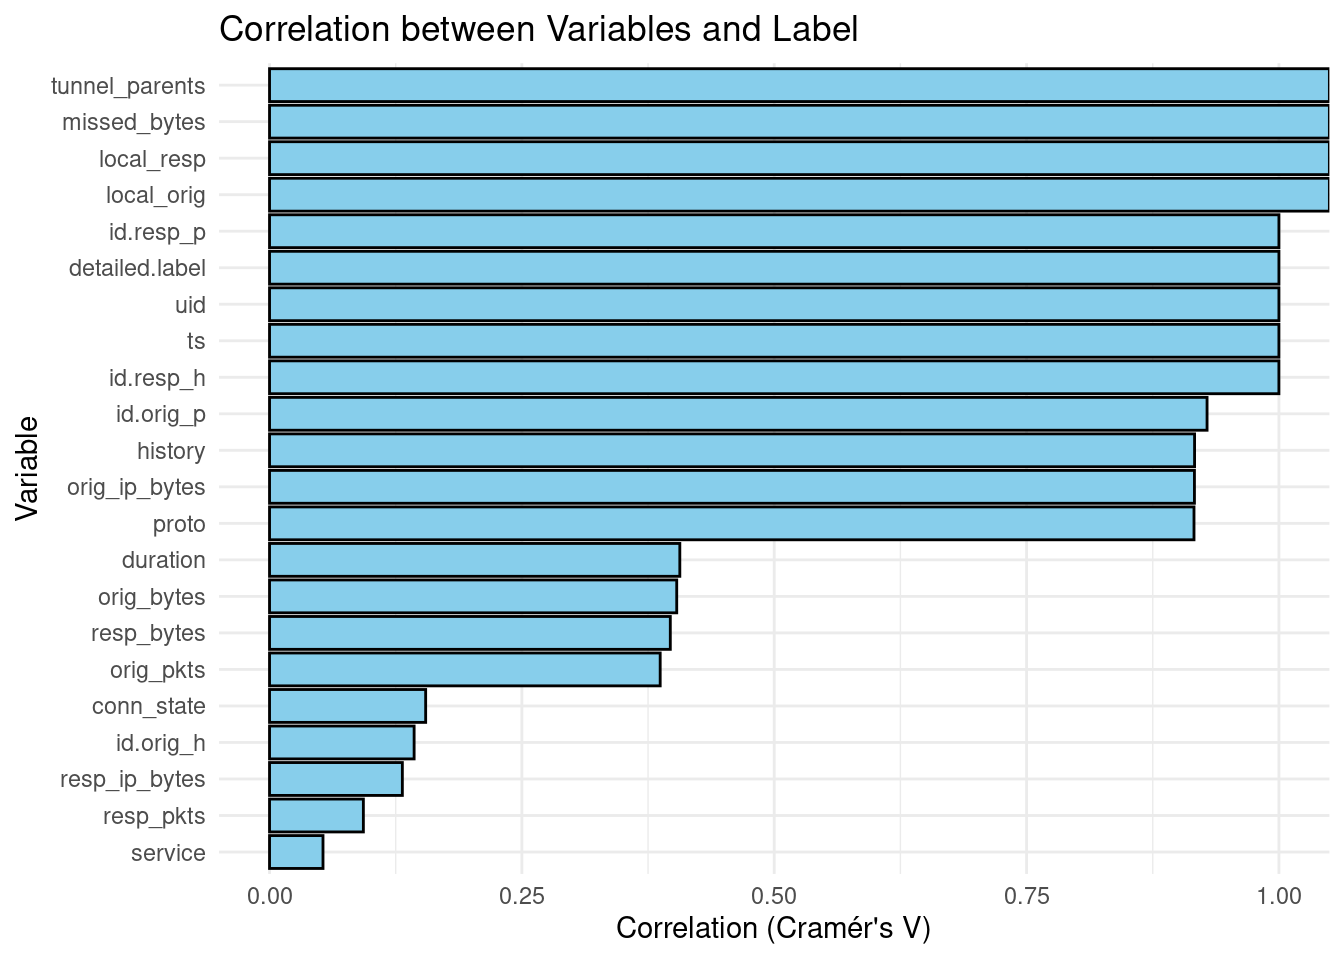
\includegraphics{Notebook_files/figure-latex/unnamed-chunk-6-1.pdf}

\hypertarget{exploring-the-categorical-variables-history-id.resp_p-id.resp_p-id.resp_h-id.resp_p-proto-all-have-high-correaltions-with-label}{%
\subsection{Exploring the Categorical Variables History, ID.Resp\_p,
ID.Resp\_p, ID.Resp\_h, ID.Resp\_p, Proto (All have high correaltions
with
label)}\label{exploring-the-categorical-variables-history-id.resp_p-id.resp_p-id.resp_h-id.resp_p-proto-all-have-high-correaltions-with-label}}

\begin{Shaded}
\begin{Highlighting}[]
\CommentTok{\# Determine the number of unique values for each variable}
\NormalTok{num\_unique\_history }\OtherTok{\textless{}{-}}\NormalTok{ attacks }\SpecialCharTok{\%\textgreater{}\%} \FunctionTok{select}\NormalTok{(history) }\SpecialCharTok{\%\textgreater{}\%} \FunctionTok{n\_distinct}\NormalTok{()}
\NormalTok{num\_unique\_id\_resp\_p }\OtherTok{\textless{}{-}}\NormalTok{ attacks }\SpecialCharTok{\%\textgreater{}\%} \FunctionTok{select}\NormalTok{(id.resp\_p) }\SpecialCharTok{\%\textgreater{}\%} \FunctionTok{n\_distinct}\NormalTok{()}
\NormalTok{num\_unique\_id\_resp\_h }\OtherTok{\textless{}{-}}\NormalTok{ attacks }\SpecialCharTok{\%\textgreater{}\%} \FunctionTok{select}\NormalTok{(id.resp\_h) }\SpecialCharTok{\%\textgreater{}\%} \FunctionTok{n\_distinct}\NormalTok{()}
\NormalTok{num\_unique\_id\_orig\_h }\OtherTok{\textless{}{-}}\NormalTok{ attacks }\SpecialCharTok{\%\textgreater{}\%} \FunctionTok{select}\NormalTok{(id.orig\_p) }\SpecialCharTok{\%\textgreater{}\%} \FunctionTok{n\_distinct}\NormalTok{()}
\NormalTok{num\_unique\_proto }\OtherTok{\textless{}{-}}\NormalTok{ attacks }\SpecialCharTok{\%\textgreater{}\%} \FunctionTok{select}\NormalTok{(proto) }\SpecialCharTok{\%\textgreater{}\%} \FunctionTok{n\_distinct}\NormalTok{()}

\CommentTok{\# Create a data frame to store the results}
\NormalTok{unique\_values\_df }\OtherTok{\textless{}{-}} \FunctionTok{data.frame}\NormalTok{(}
  \AttributeTok{variable =} \FunctionTok{c}\NormalTok{(}\StringTok{"id.resp\_p"}\NormalTok{, }\StringTok{"id.resp\_h"}\NormalTok{, }\StringTok{"id.orig\_p"}\NormalTok{, }\StringTok{"proto"}\NormalTok{, }\StringTok{"history"}\NormalTok{),}
  \AttributeTok{unique\_values =} \FunctionTok{c}\NormalTok{(num\_unique\_id\_resp\_p, num\_unique\_id\_resp\_h, num\_unique\_id\_orig\_h, num\_unique\_proto, num\_unique\_history)}
\NormalTok{)}

\CommentTok{\# Use kable for presentation}
\FunctionTok{kable}\NormalTok{(unique\_values\_df, }\AttributeTok{caption =} \StringTok{"Number of Unique Values in Each Variable"}\NormalTok{)}
\end{Highlighting}
\end{Shaded}

\begin{longtable}[]{@{}lr@{}}
\caption{Number of Unique Values in Each Variable}\tabularnewline
\toprule()
variable & unique\_values \\
\midrule()
\endfirsthead
\toprule()
variable & unique\_values \\
\midrule()
\endhead
id.resp\_p & 65426 \\
id.resp\_h & 597107 \\
id.orig\_p & 28243 \\
proto & 3 \\
history & 126 \\
\bottomrule()
\end{longtable}

\#\#Visualizing The Categorical Variables History with a WordCloud

\begin{Shaded}
\begin{Highlighting}[]
\CommentTok{\# Load necessary libraries}
\FunctionTok{library}\NormalTok{(wordcloud)}
\end{Highlighting}
\end{Shaded}

\begin{verbatim}
## Loading required package: RColorBrewer
\end{verbatim}

\begin{Shaded}
\begin{Highlighting}[]
\CommentTok{\# Filter out "unknown" values}
\NormalTok{attacks\_filtered }\OtherTok{\textless{}{-}} \FunctionTok{subset}\NormalTok{(attacks, history }\SpecialCharTok{!=} \StringTok{"unknown"}\NormalTok{)}

\CommentTok{\# Create separate datasets for malicious and benign}
\NormalTok{malicious\_data }\OtherTok{\textless{}{-}} \FunctionTok{subset}\NormalTok{(attacks\_filtered, label }\SpecialCharTok{==} \StringTok{"Malicious"}\NormalTok{)}
\NormalTok{benign\_data }\OtherTok{\textless{}{-}} \FunctionTok{subset}\NormalTok{(attacks\_filtered, label }\SpecialCharTok{==} \StringTok{"Benign"}\NormalTok{)}

\CommentTok{\# Create word cloud for malicious data}
\FunctionTok{wordcloud}\NormalTok{(malicious\_data}\SpecialCharTok{$}\NormalTok{history, }\AttributeTok{scale=}\FunctionTok{c}\NormalTok{(}\DecValTok{5}\NormalTok{,}\FloatTok{0.5}\NormalTok{), }\AttributeTok{min.freq =} \DecValTok{10}\NormalTok{, }\AttributeTok{random.order=}\ConstantTok{FALSE}\NormalTok{, }\AttributeTok{colors=}\FunctionTok{brewer.pal}\NormalTok{(}\DecValTok{8}\NormalTok{, }\StringTok{"Dark2"}\NormalTok{), }\AttributeTok{main=}\StringTok{"Malicious"}\NormalTok{)}
\end{Highlighting}
\end{Shaded}

\begin{verbatim}
## Loading required namespace: tm
\end{verbatim}

\begin{verbatim}
## Warning in tm_map.SimpleCorpus(corpus, tm::removePunctuation): transformation
## drops documents
\end{verbatim}

\begin{verbatim}
## Warning in tm_map.SimpleCorpus(corpus, function(x) tm::removeWords(x,
## tm::stopwords())): transformation drops documents
\end{verbatim}

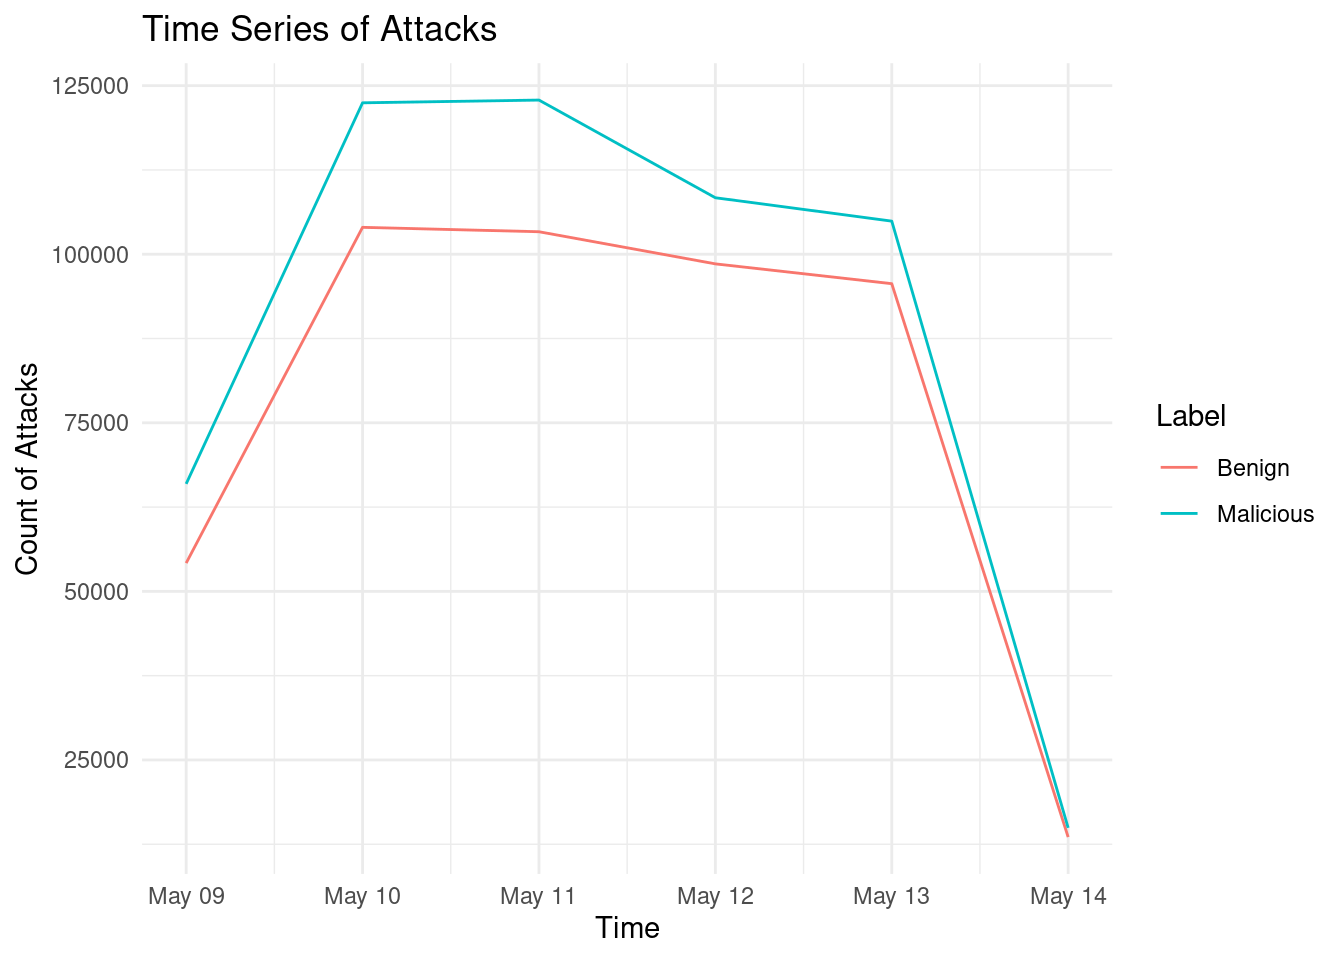
\includegraphics{Notebook_files/figure-latex/unnamed-chunk-8-1.pdf}

\begin{Shaded}
\begin{Highlighting}[]
\CommentTok{\# Create word cloud for benign data}
\FunctionTok{wordcloud}\NormalTok{(benign\_data}\SpecialCharTok{$}\NormalTok{history, }\AttributeTok{scale=}\FunctionTok{c}\NormalTok{(}\DecValTok{5}\NormalTok{,}\FloatTok{0.5}\NormalTok{), }\AttributeTok{min.freq =} \DecValTok{10}\NormalTok{, }\AttributeTok{random.order=}\ConstantTok{FALSE}\NormalTok{, }\AttributeTok{colors=}\FunctionTok{brewer.pal}\NormalTok{(}\DecValTok{8}\NormalTok{, }\StringTok{"Dark2"}\NormalTok{), }\AttributeTok{main=}\StringTok{"Benign"}\NormalTok{)}
\end{Highlighting}
\end{Shaded}

\begin{verbatim}
## Warning in tm_map.SimpleCorpus(corpus, tm::removePunctuation): transformation
## drops documents

## Warning in tm_map.SimpleCorpus(corpus, tm::removePunctuation): transformation
## drops documents
\end{verbatim}

\includegraphics{Notebook_files/figure-latex/unnamed-chunk-8-2.pdf}

\#\#Visualizing The Protocols Values on a Barchart

\begin{Shaded}
\begin{Highlighting}[]
\CommentTok{\# Ensure all varaibales are factors}
\NormalTok{attacks}\SpecialCharTok{$}\NormalTok{label }\OtherTok{\textless{}{-}} \FunctionTok{as.factor}\NormalTok{(attacks}\SpecialCharTok{$}\NormalTok{label)}
\NormalTok{attacks}\SpecialCharTok{$}\NormalTok{proto }\OtherTok{\textless{}{-}} \FunctionTok{as.factor}\NormalTok{(attacks}\SpecialCharTok{$}\NormalTok{proto)}

\CommentTok{\# Plot1 Protocols}
\FunctionTok{ggplot}\NormalTok{(}\AttributeTok{data =}\NormalTok{ attacks, }\FunctionTok{aes}\NormalTok{(}\AttributeTok{x =}\NormalTok{ proto, }\AttributeTok{fill =}\NormalTok{ label)) }\SpecialCharTok{+}
  \FunctionTok{geom\_bar}\NormalTok{(}\AttributeTok{position =} \StringTok{"dodge"}\NormalTok{) }\SpecialCharTok{+}
  \FunctionTok{labs}\NormalTok{(}\AttributeTok{title =} \StringTok{"Distribution of Labels across Protocols"}\NormalTok{,}
       \AttributeTok{x =} \StringTok{"Protocols"}\NormalTok{,}
       \AttributeTok{y =} \StringTok{"Count"}\NormalTok{) }\SpecialCharTok{+}
  \FunctionTok{scale\_fill\_brewer}\NormalTok{(}\AttributeTok{palette =} \StringTok{"Set1"}\NormalTok{)  }
\end{Highlighting}
\end{Shaded}

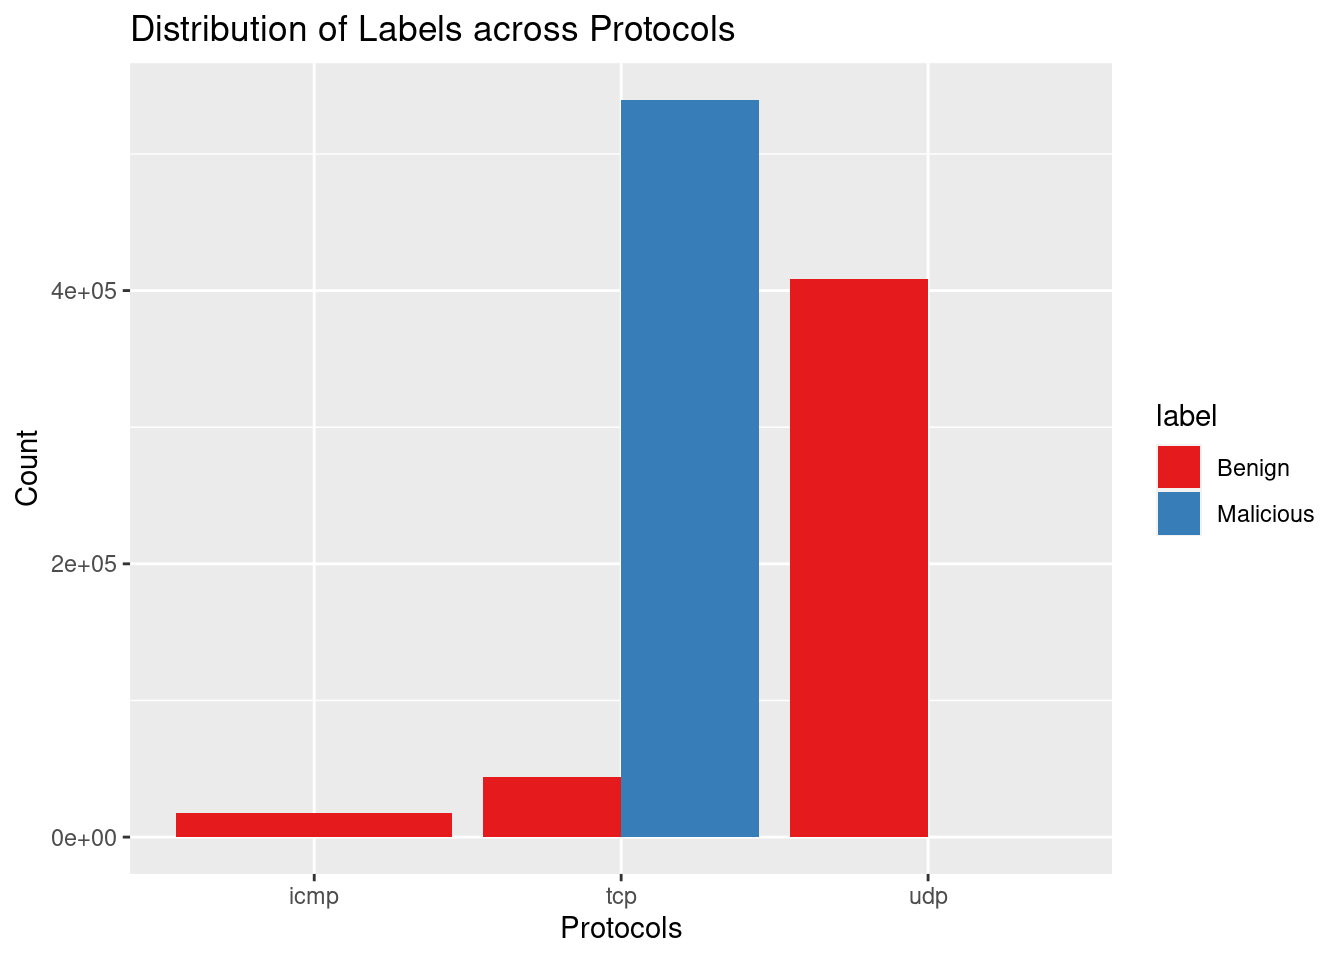
\includegraphics{Notebook_files/figure-latex/categorical-viz-1.pdf}

\hypertarget{dimensionality-reduction}{%
\subsection{Dimensionality Reduction}\label{dimensionality-reduction}}

This was the most challenging part of the project I attempted
differerent approaches like using a stepwise linear discrimination,
lemitization of IP addresses and ports to reduce dimensionality with
limited success. I opted to create a subset of the data since I was also
having problems pushing the huge original data file to Github. I decide
to create a subset of the data with only the varaibles that I was using
in my project.

\begin{Shaded}
\begin{Highlighting}[]
\CommentTok{\# Removing some of the less  important variables from the data }
\NormalTok{data1 }\OtherTok{\textless{}{-}} \FunctionTok{select}\NormalTok{(attacks, }
\NormalTok{                        label, ts, }
\NormalTok{                        id.resp\_h, id.resp\_p, id.orig\_p,}
\NormalTok{                        proto, history, orig\_ip\_bytes)}

\CommentTok{\# View the first few rows of the selected data}
\FunctionTok{summary}\NormalTok{(data1)}
\end{Highlighting}
\end{Shaded}

\begin{verbatim}
##        label              ts                          id.resp_h        
##  Benign   :469275   Min.   :2018-05-09 15:30:31.01   Length:1008748    
##  Malicious:539473   1st Qu.:2018-05-10 17:57:40.75   Class :character  
##                     Median :2018-05-11 20:40:00.00   Mode  :character  
##                     Mean   :2018-05-11 21:43:27.22                     
##                     3rd Qu.:2018-05-13 01:13:40.00                     
##                     Max.   :2018-05-14 07:24:43.02                     
##    id.resp_p       id.orig_p      proto          history         
##  Min.   :    0   Min.   :    3   icmp: 17421   Length:1008748    
##  1st Qu.:   23   1st Qu.:43730   tcp :583134   Class :character  
##  Median : 8080   Median :43763   udp :408193   Mode  :character  
##  Mean   :16098   Mean   :44437                                   
##  3rd Qu.:28180   3rd Qu.:48814                                   
##  Max.   :65535   Max.   :65394                                   
##  orig_ip_bytes    
##  Min.   :   0.00  
##  1st Qu.:  40.00  
##  Median :  60.00  
##  Mean   :  81.15  
##  3rd Qu.:  60.00  
##  Max.   :2990.00
\end{verbatim}

\hypertarget{export-the-subset-for-use-in-second-iteration-of-the-project}{%
\subsubsection{Export the Subset For Use in Second Iteration of the
Project}\label{export-the-subset-for-use-in-second-iteration-of-the-project}}

\begin{Shaded}
\begin{Highlighting}[]
\CommentTok{\#write\_xlsx(data1, path = "data/data1.xlsx") }
\CommentTok{\#Used in the first Iteration to create current Data Set}
\end{Highlighting}
\end{Shaded}

\hypertarget{separating-data-into-train-and-test}{%
\subsection{Separating Data into Train and
Test}\label{separating-data-into-train-and-test}}

The train data will be used to calibrate the data and the test will be
used to validate model predictions and generate a ROC curve.

\begin{Shaded}
\begin{Highlighting}[]
\CommentTok{\# Create a data partition}
\FunctionTok{set.seed}\NormalTok{(}\DecValTok{5774}\NormalTok{)  }
\NormalTok{trainIndex }\OtherTok{\textless{}{-}} \FunctionTok{createDataPartition}\NormalTok{(data1}\SpecialCharTok{$}\NormalTok{label, }\AttributeTok{p =} \FloatTok{0.7}\NormalTok{, }\AttributeTok{list =} \ConstantTok{FALSE}\NormalTok{, }\AttributeTok{times =} \DecValTok{1}\NormalTok{)}

\CommentTok{\# Create training and test datasets}
\NormalTok{train }\OtherTok{\textless{}{-}}\NormalTok{ data1[trainIndex, ]}
\NormalTok{test }\OtherTok{\textless{}{-}}\NormalTok{ data1[}\SpecialCharTok{{-}}\NormalTok{trainIndex, ]}

\CommentTok{\# Viewing the dimensions of the train and test sets}
\FunctionTok{dim}\NormalTok{(train)}
\end{Highlighting}
\end{Shaded}

\begin{verbatim}
## [1] 706125      8
\end{verbatim}

\begin{Shaded}
\begin{Highlighting}[]
\FunctionTok{dim}\NormalTok{(test)}
\end{Highlighting}
\end{Shaded}

\begin{verbatim}
## [1] 302623      8
\end{verbatim}

\begin{Shaded}
\begin{Highlighting}[]
\CommentTok{\# Count the number of occurrences for each level of the \textquotesingle{}label\textquotesingle{} variable}
\NormalTok{label\_counts }\OtherTok{\textless{}{-}} \FunctionTok{table}\NormalTok{(attacks}\SpecialCharTok{$}\NormalTok{label)}

\CommentTok{\# Print the counts}
\FunctionTok{print}\NormalTok{(label\_counts)}
\end{Highlighting}
\end{Shaded}

\begin{verbatim}
## 
##    Benign Malicious 
##    469275    539473
\end{verbatim}

\hypertarget{logistic-regression-model}{%
\subsection{Logistic Regression Model}\label{logistic-regression-model}}

Our Logistic Regression Model will thus use the number of bytes sent
from the origin and network protocol to determine if a network request
is malicious or benign. The base equation for this model is

\[
\begin{equation*}
\log\left(\frac{p_i}{1-p_i}\right) = \beta_0 + \beta_1 \times orig\_ip\_bytes + \beta_3 \times proto
\end{equation*}
\]\\

\begin{Shaded}
\begin{Highlighting}[]
\CommentTok{\# Running a logistic regression model with received\_callback as the response variable}
\CommentTok{\# and years\_experience, race, and gender as explanatory variables}

\NormalTok{mult\_log\_mod }\OtherTok{\textless{}{-}} \FunctionTok{glm}\NormalTok{(label }\SpecialCharTok{\textasciitilde{}}\NormalTok{ orig\_ip\_bytes }\SpecialCharTok{+}\NormalTok{ proto, }
                      \AttributeTok{data =}\NormalTok{ train, }
                      \AttributeTok{family =}\NormalTok{ binomial)}

\CommentTok{\# Displaying the summary of the model}
\FunctionTok{tidy}\NormalTok{(mult\_log\_mod)}
\end{Highlighting}
\end{Shaded}

\begin{verbatim}
## # A tibble: 4 x 5
##   term           estimate  std.error statistic  p.value
##   <chr>             <dbl>      <dbl>     <dbl>    <dbl>
## 1 (Intercept)   -17.7     35.7          -0.494 6.21e- 1
## 2 orig_ip_bytes   0.00113  0.0000775    14.5   9.60e-48
## 3 prototcp       20.1     35.7           0.561 5.74e- 1
## 4 protoudp        8.19    35.7           0.229 8.19e- 1
\end{verbatim}

\hypertarget{results}{%
\subsection{Results}\label{results}}

\hypertarget{equation-for-icmp}{%
\subsubsection{Equation for icmp}\label{equation-for-icmp}}

\[
\begin{equation*}
\log\left(\frac{p_i}{1-p_i}\right) = \beta_0 + \beta_1 \times orig\_ip\_bytes + \beta_3 \times proto
\end{equation*}
\]\\

\hypertarget{equation-for-tcp}{%
\subsubsection{Equation for TCP}\label{equation-for-tcp}}

\[
\begin{equation*}
\log\left(\frac{p_i}{1-p_i}\right) = \beta_0 + \beta_1 \times orig\_ip\_bytes + \beta_3 \times proto
\end{equation*}
\]

\hypertarget{equation-for-udp}{%
\subsubsection{Equation for UDP}\label{equation-for-udp}}

\[
\begin{equation*}
\log\left(\frac{p_i}{1-p_i}\right) = \beta_0 + \beta_1 \times orig\_ip\_bytes + \beta_3 \times proto
\end{equation*}
\]

\hypertarget{cross-validation}{%
\subsubsection{Cross Validation}\label{cross-validation}}

\begin{Shaded}
\begin{Highlighting}[]
\CommentTok{\# Create 10{-}fold cross{-}validation sets}
\FunctionTok{set.seed}\NormalTok{(}\DecValTok{123}\NormalTok{) }\CommentTok{\# for reproducibility}
\NormalTok{folds }\OtherTok{\textless{}{-}} \FunctionTok{createFolds}\NormalTok{(train}\SpecialCharTok{$}\NormalTok{label, }\AttributeTok{k =} \DecValTok{10}\NormalTok{)}

\CommentTok{\# Function to perform cross{-}validation and compute AUC for each fold}
\NormalTok{cv\_roc\_auc }\OtherTok{\textless{}{-}} \ControlFlowTok{function}\NormalTok{(train\_data, folds) \{}
\NormalTok{  auc\_list }\OtherTok{\textless{}{-}} \FunctionTok{c}\NormalTok{()}
  
  \ControlFlowTok{for}\NormalTok{(i }\ControlFlowTok{in} \DecValTok{1}\SpecialCharTok{:}\FunctionTok{length}\NormalTok{(folds)) \{}
    \CommentTok{\# Splitting data into training and test sets}
\NormalTok{    test\_indices }\OtherTok{\textless{}{-}}\NormalTok{ folds[[i]]}
\NormalTok{    train\_indices }\OtherTok{\textless{}{-}} \FunctionTok{setdiff}\NormalTok{(}\FunctionTok{seq\_len}\NormalTok{(}\FunctionTok{nrow}\NormalTok{(train\_data)), test\_indices)}
    
\NormalTok{    train\_fold }\OtherTok{\textless{}{-}}\NormalTok{ train\_data[train\_indices, ]}
\NormalTok{    test\_fold }\OtherTok{\textless{}{-}}\NormalTok{ train\_data[test\_indices, ]}
    
    \CommentTok{\# Fit the model on the training set}
\NormalTok{    glm\_model }\OtherTok{\textless{}{-}} \FunctionTok{glm}\NormalTok{(label }\SpecialCharTok{\textasciitilde{}}\NormalTok{ orig\_ip\_bytes }\SpecialCharTok{+}\NormalTok{ proto, }\AttributeTok{data =}\NormalTok{ train\_fold, }\AttributeTok{family =}\NormalTok{ binomial)}
    
    \CommentTok{\# Predict probabilities on the test set}
\NormalTok{    prob\_predictions }\OtherTok{\textless{}{-}} \FunctionTok{predict}\NormalTok{(glm\_model, }\AttributeTok{newdata =}\NormalTok{ test\_fold, }\AttributeTok{type =} \StringTok{"response"}\NormalTok{)}
    
    \CommentTok{\# Compute ROC AUC}
\NormalTok{    roc\_curve }\OtherTok{\textless{}{-}} \FunctionTok{roc}\NormalTok{(test\_fold}\SpecialCharTok{$}\NormalTok{label, prob\_predictions)}
\NormalTok{    auc\_value }\OtherTok{\textless{}{-}} \FunctionTok{auc}\NormalTok{(roc\_curve)}
\NormalTok{    auc\_list }\OtherTok{\textless{}{-}} \FunctionTok{c}\NormalTok{(auc\_list, auc\_value)}
\NormalTok{  \}}
  
  \FunctionTok{return}\NormalTok{(auc\_list)}
\NormalTok{\}}

\CommentTok{\# Perform cross{-}validation and compute AUC}
\NormalTok{auc\_results }\OtherTok{\textless{}{-}} \FunctionTok{cv\_roc\_auc}\NormalTok{(train, folds)}
\end{Highlighting}
\end{Shaded}

\begin{verbatim}
## Setting levels: control = Benign, case = Malicious
\end{verbatim}

\begin{verbatim}
## Setting direction: controls < cases
\end{verbatim}

\begin{verbatim}
## Setting levels: control = Benign, case = Malicious
\end{verbatim}

\begin{verbatim}
## Setting direction: controls < cases
\end{verbatim}

\begin{verbatim}
## Setting levels: control = Benign, case = Malicious
\end{verbatim}

\begin{verbatim}
## Setting direction: controls < cases
\end{verbatim}

\begin{verbatim}
## Setting levels: control = Benign, case = Malicious
\end{verbatim}

\begin{verbatim}
## Setting direction: controls < cases
\end{verbatim}

\begin{verbatim}
## Setting levels: control = Benign, case = Malicious
\end{verbatim}

\begin{verbatim}
## Setting direction: controls < cases
\end{verbatim}

\begin{verbatim}
## Setting levels: control = Benign, case = Malicious
\end{verbatim}

\begin{verbatim}
## Setting direction: controls < cases
\end{verbatim}

\begin{verbatim}
## Setting levels: control = Benign, case = Malicious
\end{verbatim}

\begin{verbatim}
## Setting direction: controls < cases
\end{verbatim}

\begin{verbatim}
## Setting levels: control = Benign, case = Malicious
\end{verbatim}

\begin{verbatim}
## Setting direction: controls < cases
\end{verbatim}

\begin{verbatim}
## Setting levels: control = Benign, case = Malicious
\end{verbatim}

\begin{verbatim}
## Setting direction: controls < cases
\end{verbatim}

\begin{verbatim}
## Setting levels: control = Benign, case = Malicious
\end{verbatim}

\begin{verbatim}
## Setting direction: controls < cases
\end{verbatim}

\begin{Shaded}
\begin{Highlighting}[]
\CommentTok{\# Calculate the mean AUC from all folds}
\NormalTok{mean\_auc }\OtherTok{\textless{}{-}} \FunctionTok{mean}\NormalTok{(auc\_results)}

\CommentTok{\# Output the results}
\FunctionTok{print}\NormalTok{(}\FunctionTok{paste}\NormalTok{(}\StringTok{"Mean AUC from cross{-}validation:"}\NormalTok{, mean\_auc))}
\end{Highlighting}
\end{Shaded}

\begin{verbatim}
## [1] "Mean AUC from cross-validation: 0.954349342908229"
\end{verbatim}

\hypertarget{roc-curve}{%
\subsubsection{ROC Curve}\label{roc-curve}}

\begin{Shaded}
\begin{Highlighting}[]
\CommentTok{\# First, predict the probabilities on the validation set (Split Test Data)}
\NormalTok{prob\_predictions }\OtherTok{\textless{}{-}} \FunctionTok{predict}\NormalTok{(mult\_log\_mod, }\AttributeTok{newdata =}\NormalTok{ test, }\AttributeTok{type =} \StringTok{"response"}\NormalTok{)}

\CommentTok{\# Generate the ROC object}
\NormalTok{roc\_obj }\OtherTok{\textless{}{-}} \FunctionTok{roc}\NormalTok{(test}\SpecialCharTok{$}\NormalTok{label, prob\_predictions)}
\end{Highlighting}
\end{Shaded}

\begin{verbatim}
## Setting levels: control = Benign, case = Malicious
\end{verbatim}

\begin{verbatim}
## Setting direction: controls < cases
\end{verbatim}

\begin{Shaded}
\begin{Highlighting}[]
\CommentTok{\# Plot the ROC curve}
\FunctionTok{plot}\NormalTok{(roc\_obj, }\AttributeTok{main =} \StringTok{"ROC Curve"}\NormalTok{, }\AttributeTok{col =} \StringTok{"\#1c61b6"}\NormalTok{, }\AttributeTok{lwd =} \DecValTok{2}\NormalTok{)}
\end{Highlighting}
\end{Shaded}

\includegraphics{Notebook_files/figure-latex/unnamed-chunk-13-1.pdf}

\begin{Shaded}
\begin{Highlighting}[]
\CommentTok{\# Add AUC to the plot}
\FunctionTok{auc}\NormalTok{(roc\_obj)}
\end{Highlighting}
\end{Shaded}

\begin{verbatim}
## Area under the curve: 0.9541
\end{verbatim}

\hypertarget{conlusions-and-reccommenadtions}{%
\subsection{Conlusions and
Reccommenadtions}\label{conlusions-and-reccommenadtions}}

\end{document}
